\section{Support Vector Machine}
A Support Vector Machine (SVM) is a machine learning algorithm that has been
very popular before the use of a CNN was mainstream.
Many of the texts that will be analysed later use SVMs for their classification.

A SVM works by creating an n-dimensional space, with n as the number of
inputs you have \parencite{svm}. The SVM algorithm finds the hyperplane that splits this space.
This hyperplane can then be used for classification. 
An SVM casts the problem to a higher dimensional space and this can solve a problem when the classes are not linearly separable.
This can be seen in Figure \ref{fig:svm}, where on the left there is no clear way to separate the classes but once the problem is cast to another dimensional, the separation is clear.

\begin{figure}[h]
    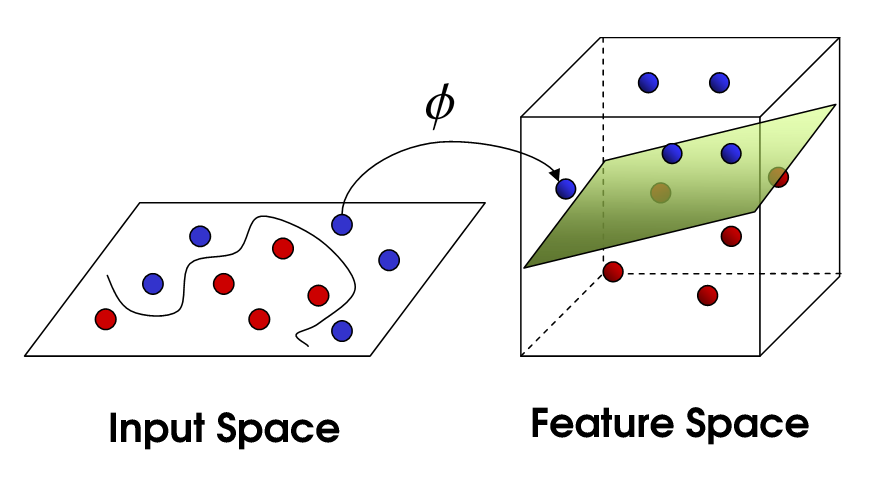
\includegraphics[scale=0.35]{svm}
    \caption{Support Vector Machine Applicability sourced from https://stackoverflow.com/questions/9480605/what-is-the-relation-between-the-number-of-support-vectors-and-training-data-and}
    \label{fig:svm}
\end{figure}

There are benefits and liabilities to using a SVM.
They can be very accurate and can work efficiently with small datasets but unfortunately it can take a large amount of time to train. 